% hakkinen-SWLBLI.tex

\section{Oblique shock boundary layer interaction.}
\label{sec:hakkinen-swlbli}
%
With some confidence that the code is working correctly and a knowledge of the 
manual postprocessing arrangements shown in the previous example,
you are ready to try to simulate a flow that has is a bit more ``realistic''.

\medskip
This is an example that introduces viscous effects but retains a very simple
geometric arrangement for the flow boundaries.
It is simple to model but immediately shows the computational demands that result
from requesting an increase in ``flow fidelity''.
Consider the Mach 2 flow of ideal air over a flat plate, 
as shown below in Figure\,\ref{fig:hakkinen-fig6b-schlieren}.
This flow image was taken as part of an experimental campaign\,\cite{hakkinen_etal_59} 
in a continuous flow wind tunnel at MIT.
The flow is from left to right in the image and the plate with the boundary layer of interest
in the lower boundary and there is a viscous-interaction shock propagating from the sharp
edge of the plate (bottom left of the image) and across the flow.
There is another plate at a small angle of attack forming the upper surface
of the test region.
The leading-edge of this shock-generator plate is out of view
but the generated shock is seen entering the field of view at the top-left of the image
and reflection from the bottom plate at approximately 49\,mm from the leading edge.
The shock reflection results in an overall pressure ratio of 1.4 across the interaction region.
The boundary layer on the plate can be seen thickening to the point of intersection with the
reflected shock and then thinning again past the interaction point.
The case for a pressure ratio of 1.4 was chosen for simulation because, as noted in the original
report\,\cite{hakkinen_etal_59}, shear-stress data indicated that the boundary layer remained laminar
after the interaction.

\begin{figure}[htbp]
 \centering
 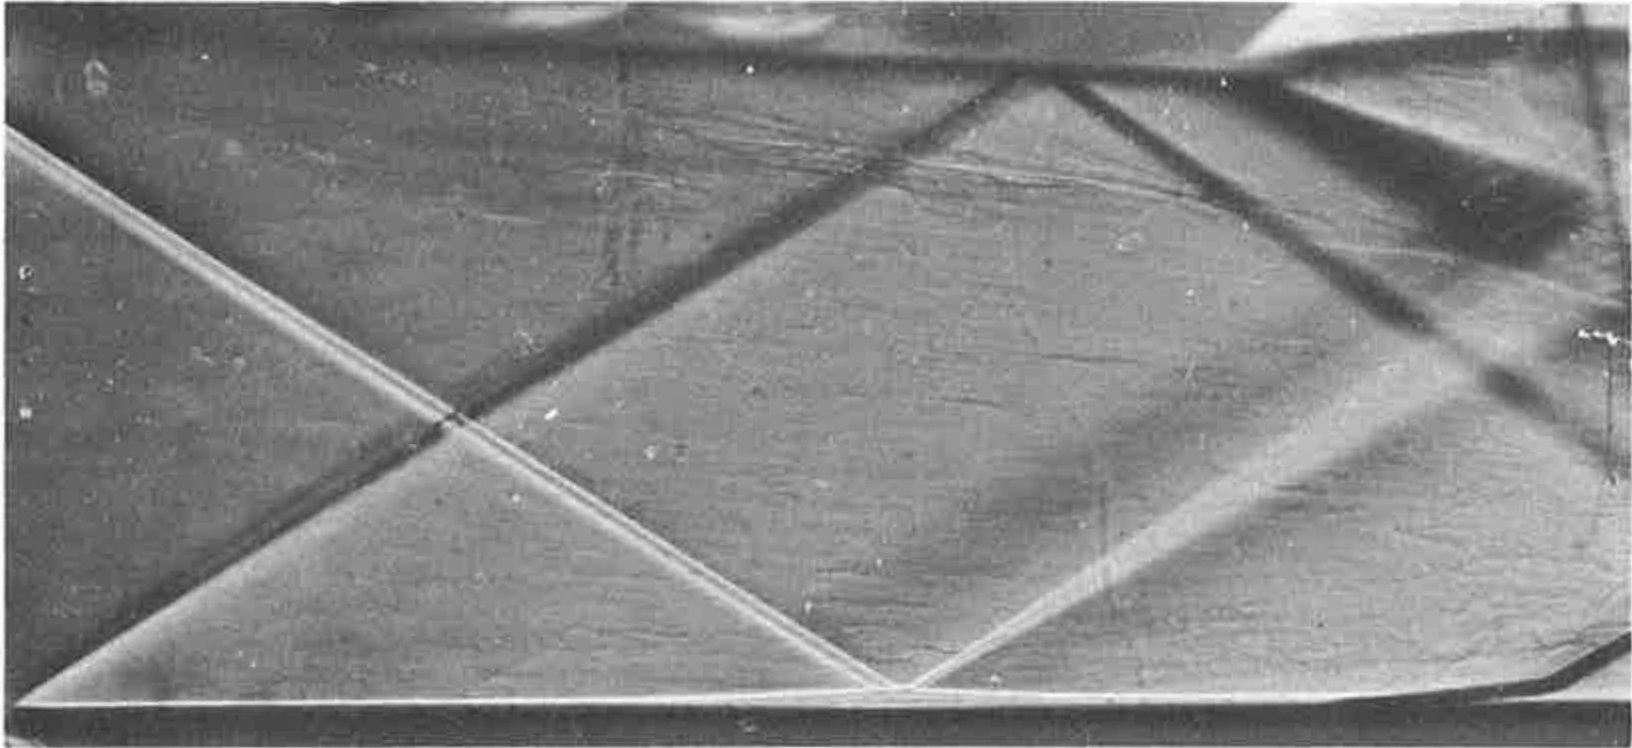
\includegraphics[width=0.7\textwidth]{../2D/hakkinen-SWLBLI/notes/fig6b-schlieren.jpeg}
 \caption{Schlieren image of the Mach 2 flow over a flat plate taken 
          from Fig.6b in Reference\,\cite{hakkinen_etal_59}.}
 \label{fig:hakkinen-fig6b-schlieren}
\end{figure}

\medskip
Although the behaviour of laminar compressible-flow boundary layers on flat plates are well predicted 
via simple theories, the addition of an impinging shock significantly more difficult to analyse manually.
The flow complexity significantly while the defining flow geometry remains very simple. 

\bigskip
\subsection{Input script (.py)}
%
Figure\,\ref{fig:hakkinen-geometry} shows the region, as modelled for simulation.
The flat plate is truncated at the length seen in the experimental flow image even though
the actual plate extended for 8 inches in the experiment.
Also the shock generator plate is modelled as an idealized, inviscid wall, even though
the real shock generator would have had a boundary layer and associated viscous interaction
at its leading edge.
It has been convenient to apply a slip-wall boundary condition at the shock generator
surface so that the calculation to estimate the deflection angle for the specified
pressure rise across the reflected shock uses just the usual oblique-shock relations
for an ideal gas.
Using the cfpylib ideal-flow functions in the following script and a minute of trial and error fiddling, 
the shock generator deflection angle can be estimated as being 3.09$^o$.
\index{cfpylib!ideal gas relations!example of use}
\topbar
\lstinputlisting[language={}]{../2D/hakkinen-SWLBLI/notes/double_oblique_shock.py}
\bottombar

\begin{figure}[htbp]
 \centering
 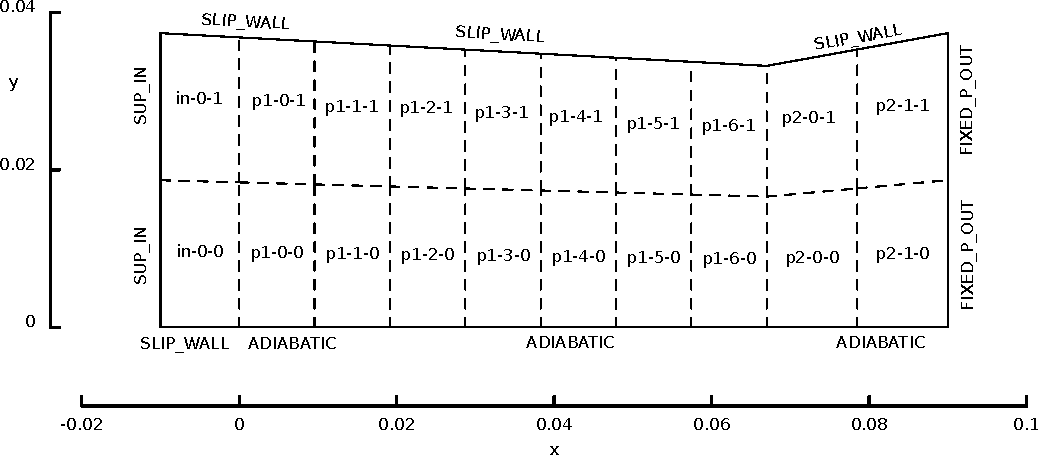
\includegraphics[width=\textwidth]{../2D/hakkinen-SWLBLI/swlbli-edited.pdf}
 \caption{Schematic view of the simulated flow region for the shock-wave interaction 
          with a laminar boundary layer.}
 \label{fig:hakkinen-geometry}
\end{figure}

\medskip
In the input script, geometric dimensions of the flow region and plate are simply scaled
from the flow image and the shock location identified in the associated pressure and skin-friction plot.
The flow region is modelled as a box with straight-line boundary segments and,
although the geometry is particularly simple, we use a three SuperBlock2D objects to split the region
into 20 individual blocks.\index{block!SuperBlock2D!example of use}
This is done so that these blocks may be assigned to several processors of a multicore machine and we
don't have to wait quite so long for our simulation to run.

\medskip
Using data in the original report\,\cite{hakkinen_etal_59}, the free-stream conditions for Fig.6b 
with $Re_{x-shock} = 2.96 \times 10^5$,
can be estimated to be $p_{\infty} = 6.205$\,kPa, $T_{\infty} = 164.4$\,K and $u_{\infty} = 514$\,m/s 
for ideal air with $R_{gas}$=287\,J/kg$\cdot$K and $\gamma$=1.4.

\noindent
\topbar
\lstinputlisting[language={}]{../2D/hakkinen-SWLBLI/swlbli.py}
\bottombar


\bigskip
\subsection{Running the simulation}
%
To get the simulation started, try the following commands:\\
%
\topbar\\
\texttt{\$ cd $\sim$/cfcfd3/examples/eilmer3/2D/hakkinen-SWLBLI/}\\
\texttt{\$ ./prep.sh}\\
\texttt{\$ ./run.sh}\\
\texttt{\$ tail -f run.transcript}\\
\bottombar\\
%
You should see the usual console output of a simulation proceeding to take time steps
and reporting it's progress toward reaching a final time.
If you are working on a 4-core machine, go and have dinner and return
in about 5 hours to check the state of the simulation.
The grid and initial solution are created with the \texttt{prep} script
and the time-evolution of the flow field is then computed for about 876\,$\mu$s 
(with 11186 time steps being required).
At the end of this pass of the simulation, it turns out that 
the separation region is still slightly evolving as indicated by small movements of the waves
propagating from that region.
We restart the calculation\index{restart!example of use}
and run it to twice the original value of \verb!max_time!.
This is achieved by manually editing the \texttt{swlbli.control} file
as described in Section\,\ref{sec:restart-sim} and setting
\verb!max_time = 1.750972e-03! and \verb!dt = 8.000000e-08! then running the command:
\topbar\\
\texttt{\$ ./run-2.sh}\\
\bottombar\\
The commands invoke the shell scripts displayed in 
subsection~\ref{hakkinen-sh-files}.

\subsection{Results}
%
Figure\,\ref{fig:hakkinen-field-data} shows some of the flow field data at $t$=1.75\,ms after flow start.
The magnitude of the gradients of density (Fig.\,\ref{fig:hakkinen-gradient}) are also shown 
as an approximation to the schlieren image of Figure\,\ref{fig:hakkinen-fig6b-schlieren}.

\begin{figure}[htbp]
 \centering
 \subfloat[Pressure field.]{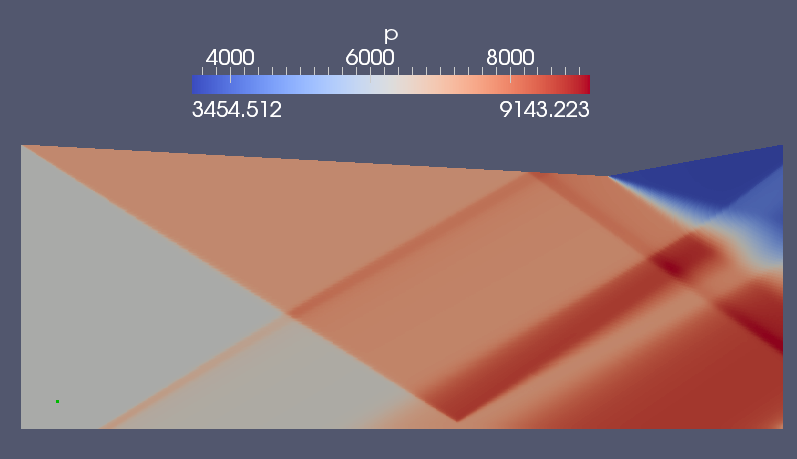
\includegraphics[width=0.7\textwidth]
    {../2D/hakkinen-SWLBLI/p-field-1p75ms.png}\label{fig:hakkinen-pressure}}\\
 \subfloat[Temperature field.]{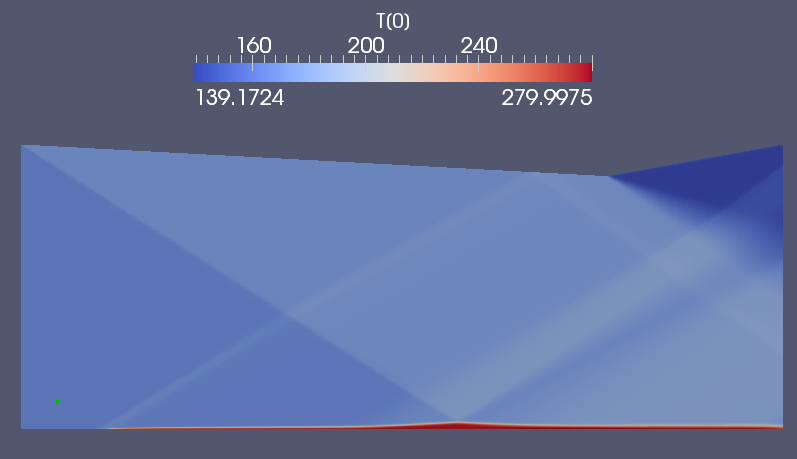
\includegraphics[width=0.7\textwidth]
    {../2D/hakkinen-SWLBLI/t-field-1p75ms.png}\label{fig:hakkinen-temperature}}\\
 \subfloat[Gradient of density field.]{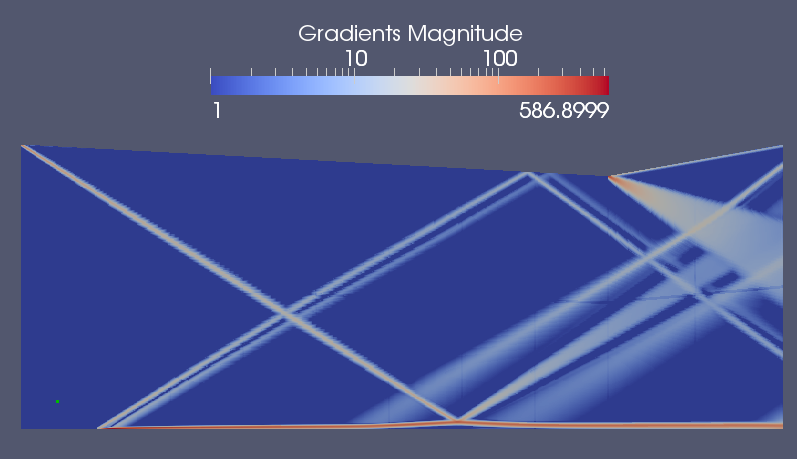
\includegraphics[width=0.7\textwidth]
    {../2D/hakkinen-SWLBLI/rho-gradients-1p75ms.png}\label{fig:hakkinen-gradient}}
 \caption{Computed flow field at $t$=1.75\,ms.}
 \label{fig:hakkinen-field-data}
\end{figure}

\medskip
The real proof of success is in comparison with the experimental data.
Figure\,\ref{fig:hakkinen-plate-data-compare} shows the pressure and shear-stress along the plate.
The simulation has done a reasonable job of estimating the pressure distribution right 
through the separation zone.
Features that look a little wrong include the viscous interaction region at $x$=0,
which is a bit extended because of lack of resolution at the start of the boundary layer.
Also, there is an artificial drop in pressure at the right end of the simulation domain
where the boundary layer exits the flow domain but this is of no concern because  
the flat plate used in the experiment was more than twice the length of this simulated version.

\medskip
The simulation has done a reasonable job on the shear stress,
which has been computed from the field data using the script in Section\,\ref{hakkinen-post-processing}.
This quantity is difficult to compute and difficult to measure so it is reassuring that both
sets of data line up nicely with the Blasius value in the boundary layer leading into the interaction region.
After the interaction region, the computed values recover to the Blasius level 
just before rising toward the end of the flow domain.
This is, again, the interaction with the outflow boundary condition and would be removed from view
if the full length of the plate was simulated.

\begin{figure}[htbp]
 \centering
 \subfloat[Pressure.]{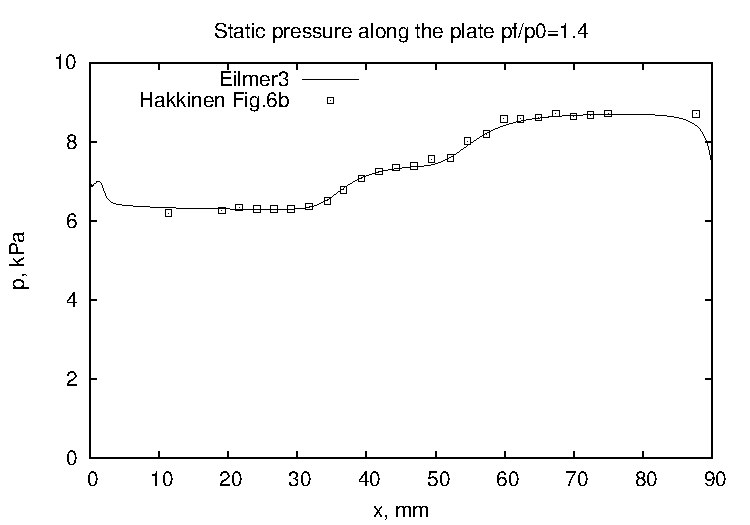
\includegraphics[width=0.5\textwidth]
    {../2D/hakkinen-SWLBLI/pressure.pdf}\label{fig:hakkinen-pressure-on-plate}}
 \subfloat[Shear stress.]{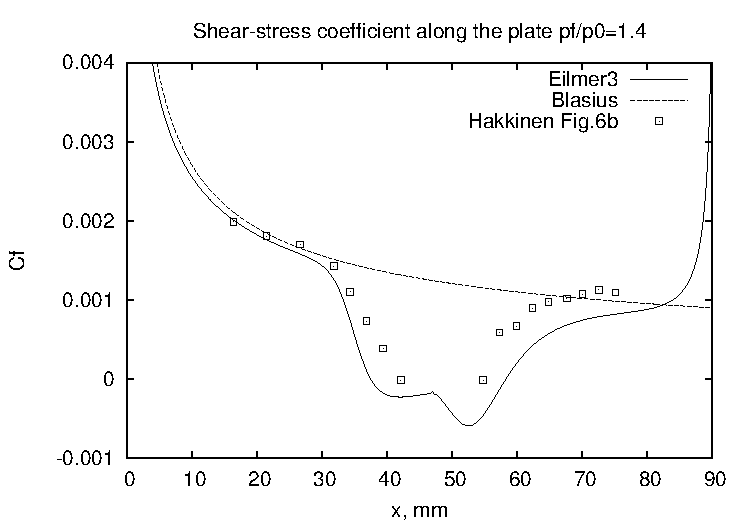
\includegraphics[width=0.5\textwidth]
    {../2D/hakkinen-SWLBLI/shear.pdf}\label{fig:hakkinen-shear-stress-on-plate}}
 \caption{Distribution of pressure and shear along the plate at $t$=1.75\,ms.}
 \label{fig:hakkinen-plate-data-compare}
\end{figure}

\subsection{Shell scripts}
\label{hakkinen-sh-files}
\topbar
\lstinputlisting[language={}]{../2D/hakkinen-SWLBLI/prep.sh}
\bottombar\\
\topbar
\lstinputlisting[language={}]{../2D/hakkinen-SWLBLI/run.sh}\index{mpimap!example of use}
\bottombar\\
\topbar
\lstinputlisting[language={}]{../2D/hakkinen-SWLBLI/run-2.sh}
\bottombar\\
\topbar
\lstinputlisting[language={}]{../2D/hakkinen-SWLBLI/post.sh}
\bottombar\\
\topbar
\lstinputlisting[language={}]{../2D/hakkinen-SWLBLI/plot.sh}
\bottombar

\subsection{Postprocessing for shear stress}
\label{hakkinen-post-processing}
%
The script below uses the functions imported from \texttt{e3\_flow.py}
at a slightly higher level than in the cone20 example.
It extracts the data for the cell nearest to the flat plate and uses that data
to compute the expected shear stress on the plate.

\noindent
\topbar
\lstinputlisting[language={}]{../2D/hakkinen-SWLBLI/compute_shear.py}
\bottombar

\subsection{Notes}
\begin{itemize}
 \item The influence of the flat plate boundary layer on the pressure 
   in the region near the plate is small but measureable.
   With a free-stream pressure of 6.205\,kPa specified at the inflow plane,
   we see 6.28\,kPa in the pressure data leading into the shock-interaction region.
   For the free-stream conditions used, the displacement thickness of a simple
   flat-plate boundary layer would be expected to be approximately 0.112\,mm
   at 25\,mm from the leading edge of the plate.
   If this displacement effect could be modelled as a straight wedge deflecting the
   inviscid free-stream, the corresponding oblique shock would have 
   a static pressure ratio of 1.0146.
   This gives an expected pressure of 6.295\,kPa in the boundary-layer external flow
   leading into the shock interaction, quite close to the simulation value. 
\end{itemize}
